%%% -*- TeX-engine: xetex -*-
\documentclass{beamer}

% for themes, etc.
\usepackage{times}  % fonts are up to you
\usepackage{graphicx}
\usepackage{color}
\usepackage{hyperref}

\mode<presentation>
{
  \usetheme{Warsaw}
  \useoutertheme{infolines}
  \usecolortheme{whale}
  \setbeamertemplate{navigation symbols}{}
}
\usepackage{fontspec}
\usepackage{xunicode}
\usepackage[BoldFont,SlantFont]{xeCJK}
\setCJKmainfont{SimSun}
\setCJKmonofont{SimHei}

\title{
  基于翻译技术的流量调度研究 \\
  结题报告
}
\author{王文鑫}
\date{2016年6月8日}

\begin{document}

\begin{frame}
  \titlepage
\end{frame}

\section{研究课题}

\begin{frame}
  \frametitle{研究课题}

  在IPv4/IPv6过渡场景中,基于翻译等过渡技术,\\设计和实现灵活通用的流量调度机制,\\
  使得ISP可以自由定制多出口情景下的调度策略
\end{frame}

\section{研究背景}
\subsection{IPv4/IPv6过渡}
\begin{frame}
  \frametitle{IPv4和IPv6}

  \begin{block}{IPv4}
    \begin{itemize}
    \item 地址数量有限:$2^{32} \doteq 43$亿地址,已于2011年2月3日枯竭\footnotemark[1]
    \end{itemize}
  \end{block}

  \begin{block}{IPv6:吸取了IPv4的经验和教训}
    \begin{itemize}
    \item 地址数量巨大:$2^{128} \doteq 10^{38}$个地址
    \item 简化数据格式、配置和路由表,提高效率:
      \begin{itemize}
      \item IP包头:去除了校验码等信息,提高处理效率
      \item 地址配置:利用设备标识自动配置全局可达地址,简化管理
      \item 全局路由表:采用高度聚类的前缀分配原则,提高路由匹配效率
      \end{itemize}
    \item 原生的多播支持、端到端透明、强制IPSec支持……
    \end{itemize}
  \end{block}
  \footnotetext[1]{https://www.nro.net/news/ipv4-free-pool-depleted}
\end{frame}

\begin{frame}
  \frametitle{过渡技术}

  \begin{block}{IPv6不兼容IPv4}
    \begin{itemize}
    \item IPv4到IPv6的切换是一个渐进的过程
      \begin{itemize}
      \item IPv6诞生20周年:扩展迅速,全球覆盖率未过半\footnotemark[1]
      \end{itemize}
    \item 在很长的一段时间内,IPv4和IPv6网络共存
    \item 不同IP协议的用户访问不同IP协议的网络资源
    \end{itemize}
  \end{block}
  \begin{block}{过渡技术}
    \begin{itemize}
    \item 保证升级过程中对原始IPv4应用的支持
    \item 跨越不同IP协议访问网络资源
    \end{itemize}
  \end{block}
  \footnotetext[1]{https://www.google.com/intl/en/ipv6/statistics.html}
\end{frame}

\begin{frame}
  \frametitle{课题研究的过渡场景}

  \vspace{1em}

  \begin{block}{}
    \begin{itemize}
    \item 所有流量必须先通过IVI无状态翻译
    \item DS-Lite隧道仅作为无法翻译时的后备方法
    \item 出口闲置
    \end{itemize}
  \end{block}
\end{frame}

\subsection{流量调度}
\begin{frame}
  \frametitle{原因}

  \vspace{1em}

  \begin{block}{}
    \begin{itemize}
    \item 所有流量必须先通过IVI无状态翻译
    \item DS-Lite隧道仅作为无法翻译时的后备方法
    \item 出口闲置
    \end{itemize}
  \end{block}
\end{frame}

\begin{frame}
  \frametitle{目标}

  \vspace{1em}

  \begin{block}{}
    \begin{itemize}
    \item 所有流量必须先通过IVI无状态翻译
    \item DS-Lite隧道仅作为无法翻译时的后备方法
    \item 出口闲置
    \end{itemize}
  \end{block}
\end{frame}

\subsection{内容和意义}
\begin{frame}
  \frametitle{目标模型}

  \begin{block}{}
    \begin{itemize}
    \item 按照流信息、链路状态等参数向不同出口分发流量
    \end{itemize}
  \end{block}
\end{frame}

\section{翻译器设计}
\begin{frame}
  \frametitle{翻译器设计}

  \begin{block}{模块}
    \begin{itemize}
    \item 控制器:观察、决策
    \item OVS交换机:分发,非传统路由,可编程性强
    \item 翻译/隧道出口选择 $\rightarrow$ 流表项
    \item netns封装:隔绝调度和出口路由
    \end{itemize}
  \end{block}
\end{frame}

\section{完成工作}
\begin{frame}
  \frametitle{完成工作}

  \begin{block}{}
    \begin{itemize}
    \item 使用libvirt和netns搭建环境,测试拓扑设计和代码
    \item OVS:设计流表
    \item 翻译器:netfilter $\rightarrow$ iptables,可以被netns隔离
    \item 控制器:静态策略、轮询切换
    \end{itemize}
  \end{block}
\end{frame}

\begin{frame}
  \frametitle{实验平台}

  \begin{center}
    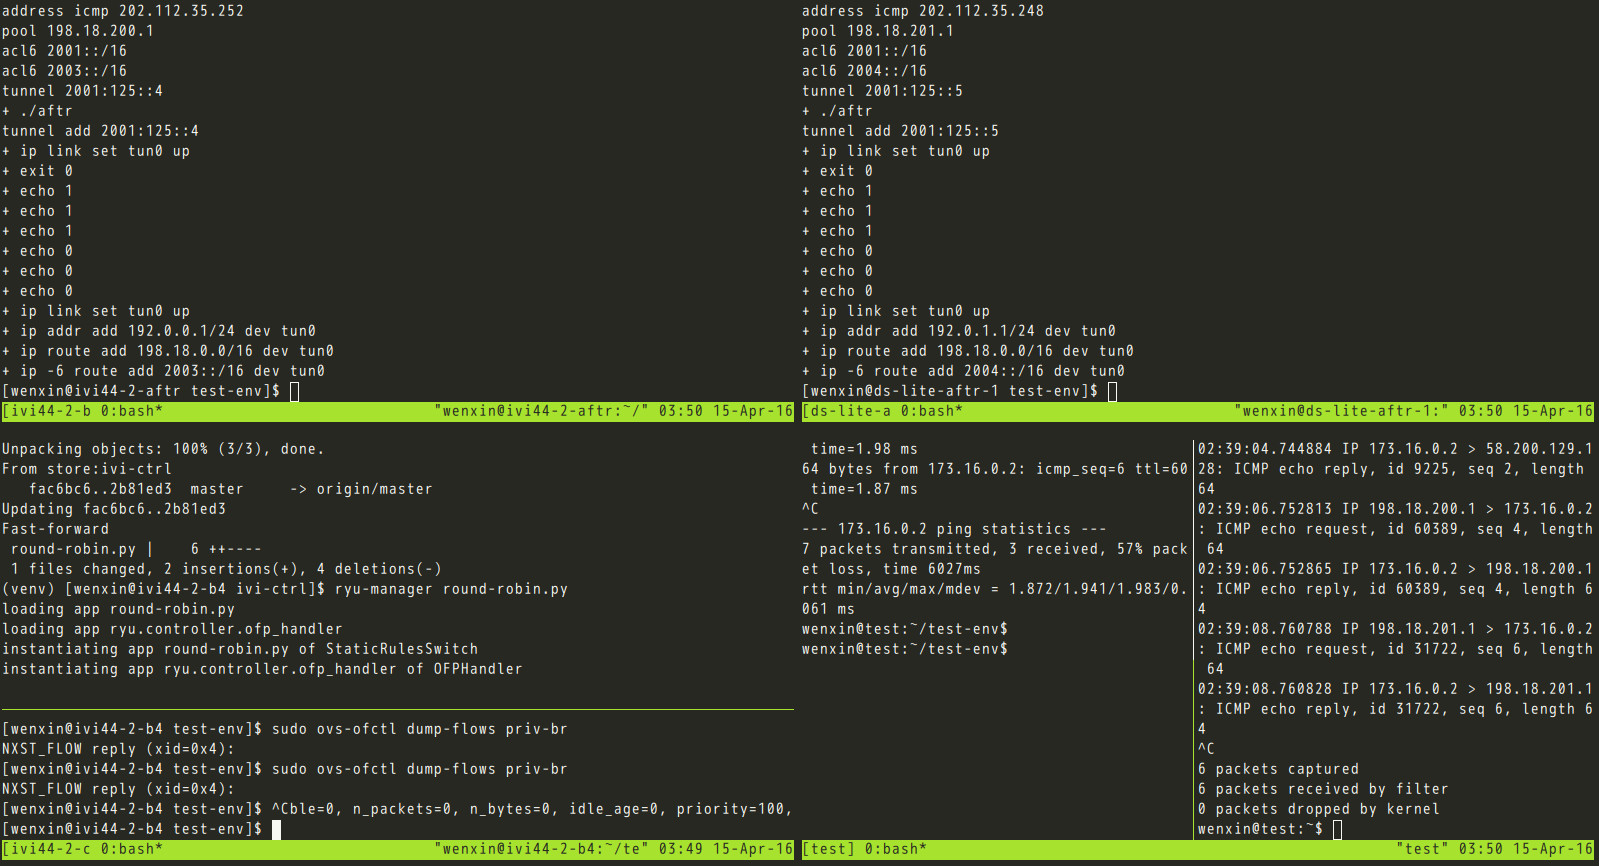
\includegraphics[width=\textwidth]{figs/test-env.jpeg}
  \end{center}
\end{frame}

\begin{frame}
  \frametitle{控制器}

  \begin{center}
    \includegraphics[width=\textwidth]{figs/static.jpeg}
  \end{center}

  \begin{center}
    \includegraphics[width=\textwidth]{figs/round-robin.jpeg}  
  \end{center}
  
\end{frame}

\section{后续工作}
\begin{frame}
  \frametitle{后续工作}

  \begin{block}{}
    \begin{itemize}
    \item 在多个二级翻译器间控制调度
    \item 添加NAT64隧道
    \end{itemize}
  \end{block}
\end{frame}

\section{进度安排}

\begin{frame}
  \frametitle{进度安排}
  \begin{block}{}
    \begin{itemize}
    \item 4月15日-5月15日:实现多个翻译器间的调度
    \item 5月16日-答辩:封装接口,完善论文
    \end{itemize}
  \end{block}
\end{frame}

\section{参考文献}
\begin{frame}
  \frametitle{参考文献}
  \begin{itemize}
  \item \href{https://tools.ietf.org/html/rfc7599}{RFC7599}
  \item \href{https://tools.ietf.org/html/rfc7597}{RFC7597}
  \item \href{https://tools.ietf.org/html/rfc6219}{RFC6219}
  \item \href{https://tools.ietf.org/html/rfc6052}{RFC6052}
  \item \href{https://tools.ietf.org/html/rfc7598}{RFC7598}
  \item
    \href{http://openvswitch.org/}{Open vSwitch}
  \item
    \href{http://osrg.github.io/ryu/}{Ryu component-based software defined networking framework }
  \end{itemize}
\end{frame}

\section{Q\&A}

\begin{frame}
  \frametitle{Q\&A}
  \begin{center}
    {\LARGE 谢谢!}
    \vspace{3em}
    {\LARGE 请老师们提问和指导!}
  \end{center}
\end{frame}
\end{document}